\chapter{Introduction}

The introduction should attempt to set your work in the context of other work done in the field. It
should demonstrate that you are aware of what you are doing, and how it relates to other work
(with references). It should also provide an overview of the contents of the project. You should
highlight your individual contributions and any novel result: which of the calculations, theorems,
examples, proofs, conjectures, codes etc. are your own?


\begin{figure}[b!] %Use h,t,b,! to enforce the location of the figure
    \centering
    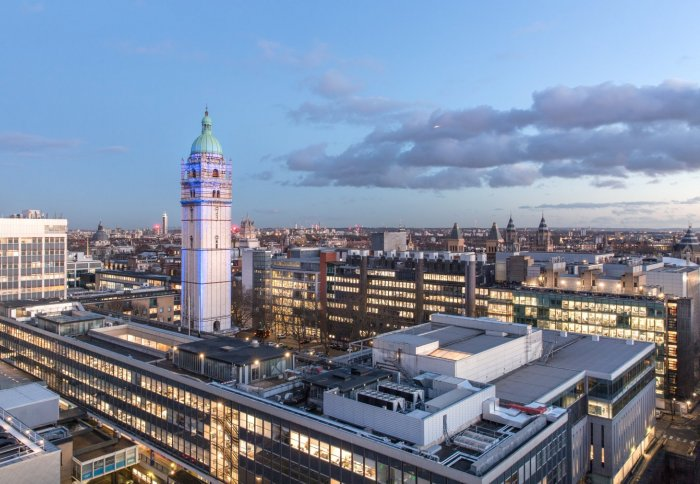
\includegraphics[width=0.8\textwidth]{Figures/imperial.jpg}
    \caption{This is an example of how you include a figure with a descriptive caption. This is an image of the South Kensington campus of Imperial College London on which we can recognize Queen's tower.}
    \label{fig:imperial-picture}
\end{figure}

Here is some filler text to show you what a few pages may look like. 
\lipsum[2-4] See Figure \ref{fig:imperial-picture}. \textbf{This is how you reference your figure in the text.}

\begin{table}[]
    \centering
    \begin{tabular}{llr}  
        \toprule
        \multicolumn{2}{c}{Module} \\
        \cmidrule(r){1-2}
        Module code    & Module name & Number of students \\
        \midrule
              & per gram    & 13.65      \\
                      &    each     & 0.01       \\
        Gnu       & stuffed     & 92.50      \\
        Emu       & stuffed     & 33.33      \\
        Armadillo & frozen      & 8.99       \\
        \bottomrule
    \end{tabular}
    \caption{Example booktabs table. Booktabs tables are nicer than regular ones. This site has a nice GUI for making LaTeX tables, and has a Booktabs option: https://www.tablesgenerator.com/}
    \label{tab:my_label}
\end{table}

\lipsum[1-4] \textbf{This is how you would reference a table:} Table \ref{tab:my_label}. 

\section{Section Example}
\label{sec:sec_example}
\lipsum[1]
\subsection{Subsection Example}
\label{sec:subsec_example}
\lipsum[1]

\subsubsection{Subsubsection Example}

Note that you can reference chapters, sections, subsections and subsubsections. For example: Subsection \ref{sec:subsec_example}!

\section{Math Example}

While math can be written inline like so $f(x) = \sum_{n=0}^{\infty} \frac{x^n}{n!}$, we often need to write stand-alone equations like so
\begin{equation}
\textrm{score}(x) = \left(\lambda_m\sum_{i=0}^{|\mathbf{m}|} \log \hat{p}_m(d(x, \mathbf{m}_i) \mid l_i)\right) + \left(\lambda_l\sum_{i=0}^{|\mathbf{l}|} \log\hat{p}_l(d(x, \mathbf{l}_i) \mid \mathbf{v}_i)\right) + \lambda_p \hat{p}_p(x)
\end{equation}

To write equations over multiple lines (like systems of equation or equations too long to fit the page), one can use the \textit{align} environment coupled to the \textit{subequations} environment like so
\begin{subequations}
\begin{align}
    \mathbb{P}(0 \leadsto -a) &= D\int_0^\infty dt\, k_r e^{-k_r t}\int_0^t d\tau\,\partial_x u \big|_{x=-a}, \\
    \mathbb{P}(0 \leadsto b) &= -D\int_0^\infty dt\, k_r e^{-k_r t}\int_0^t d\tau\,\partial_x u \big|_{x=b}.
\end{align}
\end{subequations}

\section{Algorithm Example}

See Algorithm \ref{algorithm:posit}

\begin{algorithm}[]
\SetAlgoLined
\SetKwInOut{KwInput}{Input}
\SetKwInOut{KwOutput}{Output}
\SetKwInOut{KwPre}{Pre}
\SetKw{Return}{return}
\SetKwProg{Fn}{Function}{}{end}
\LinesNumbered
\KwInput{$\textbf{m}$, such that $\mathbf{m}_i$ is the position of the $i$'th monitor\newline
$\textbf{l}$, such that $\mathbf{l}_i$ is the position of the $i$'th landmark\newline
$\mathbf{p}^m$, such that $\mathbf{p}^m_i$ is the ping latency from monitor $i$ to the target\newline
$\mathbf{p}^l$, such that $\mathbf{p}^l_i$ is the set of ping latencies to landmark $i$}

\BlankLine
\KwPre{Compute $\hat{p}_m(d \mid l)$, an estimator giving the likelihood of the target being distance $d$ away from the monitor, given that the monitor records a latency of $l$ to that target. Implemented by training a KDE using $\mathbf{p}^l$.\newline
Compute $\hat{p}_l(d \mid v)$, an estimator giving the likelihood of the target being distance $d$ away from the landmark, given a Canberra distance of $v$ between the target and the landmark, using training targets.
}
\BlankLine
\KwOutput{Most likely location of the target}
\BlankLine

\Fn{Likelihood($x$, $\mathbf{v}$)} {
MonitorScore $\gets \sum_{i=0}^{|\mathbf{m}|} \log{\hat{p}_m(d(x, \mathbf{m}_i) \mid l_i)}$\;
LandmarkScore $\gets \sum_{i=0}^{|\mathbf{l}|} \log{\hat{p}_l(d(x, \mathbf{l}_i) \mid \mathbf{v}_i)}$\;
\Return MonitorScore + LandmarkScore
}

\BlankLine
$\mathbf{v} \gets $\{$\mathrm{canberra\_distance}(\mathbf{l}_i, \mathbf{p}^m) \mid \mathbf{l}_i \in \mathbf{l}$\}

$\mathbf{C}$ $\gets$ Constraint-Based-Geolocation($\mathbf{m}$, $\mathbf{p}^m$)\;
$\mathbf{C_l}$ $\gets$ \{$m \in \mathbf{m} \mid \mathbf{C}$ contains $m\} \cup \{l \in \mathbf{l} \mid \mathbf{C}$ contains $l$\}\;
\BlankLine
\Return argmax$_{x\in \mathbf{C_l}}$ Likelihood($x$)

 \caption{Algorithm example}
 \label{algorithm:posit}
\end{algorithm}


\section{Reference Example}

Here is how you can cite papers which you have added in the \verb!/bibs/bibliography.bib! file. You can cite single references as such \cite{Einstein1905} or multiple references like so \cite{Dirac1981,Einstein1905}. Here is a reference to a website \cite{Riemann2024}.
